\section{これまでの結果}

\begin{frame}{周期外力付き Rössler 方程式(1/2)}        
    \begin{minipage}{0.4\textwidth}
            \begin{figure}
                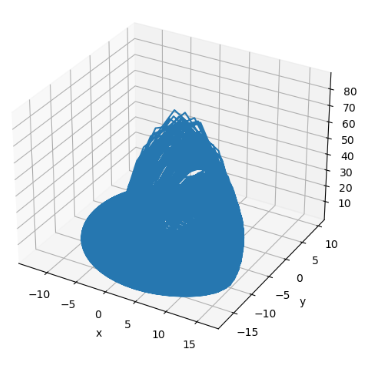
\includegraphics[width=0.7\textwidth]{Fig/Rossler_attractor.png}
                \caption{位相シフトのある周期外力付きのRössler システム}
                \label{rossler_attractor.png} % ラベルを付ける(参照する場合に使用)
            \end{figure}
            \vspace{-.7cm}
            \begin{itemize}
                \item 位相シフト(クロニックジェットラグ)を含む周期外力がある系の予測を Reservoir Computer で行う:
            \end{itemize}
        \end{minipage}
    \begin{minipage}{0.59\textwidth}
        \vspace{-1.0cm}
        \begin{align}
            \frac{dx}{dt} &= -y - z + A \sin(t + \theta_p(t))\\
            \frac{dy}{dt} &= x + ay \\
            \frac{dz}{dt} &= b + z(x - c)
        \end{align}
        \vspace{-.5cm}
        \begin{itemize}
            \item 学習と予測は,$x,\ y,\ A \sin(t + \theta_p(t))$ を対象とする.
            \item 外力の振幅$A = 2.0$,変数$a = 0.2,\ b = 0.2,\ c = 5.7$,初期条件$ \left[ x, y, z \right] = [1.0, 1.0, 1.0]$.時間範囲:$[0, 2510]$, 系の周期は $2\pi$ .
            \item $\theta_p(t)$ は$t$について定期的に位相シフトを与える関数.ここでは,まず$p \in \left\{ n \in \Z \mid -12 \leq n \leq 12 \right\}$をとり,$4$ 日に一度 $p \cdot 2\pi/24$ だけ系を早めるようなものとする.    
        \end{itemize}
    \end{minipage}
\end{frame}

\begin{frame}{周期外力付き Rössler 方程式(2/2)}
    \begin{figure}
        %\centering % 画像を中央揃えにする(オプション)
        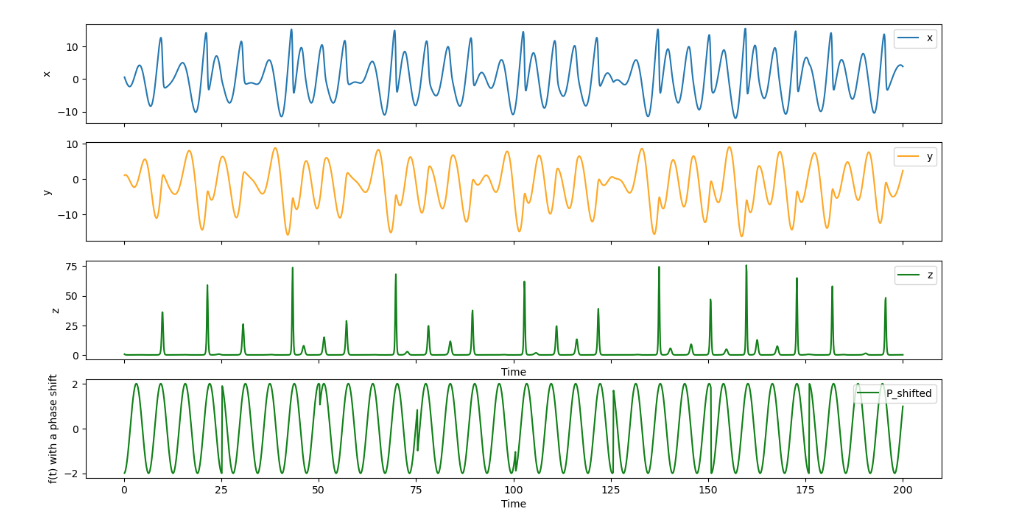
\includegraphics[width=0.75\textwidth]{Fig/Plot_rossler_variables.png}
        \caption{位相シフトのある周期外力付きのRössler システム:\\変数ごとと外力の時系列のグラフ}
        \label{plot_rossler_attractor.png} % ラベルを付ける(参照する場合に使用)
    \end{figure}
\end{frame}


\begin{frame}{Reservoir Computerによる予測:手法}
    $\triangle t = 0.1$ とした.
    \begin{itemize}
        \item Hyperparametersの最適化
        \begin{itemize}
            \item 学習期間: Rössler システムにおける $z$ 変数が観測できないものとして, $x, y$ 変数 と 外力 $f(t)$ を入力する.期間は $\left.\left[ 0, 1000 \right.\right).$ \vspace{.2em}
            \item 損失関数を学習期間全体に対して定義された nrmse として最適化:
            \vspace{.2em}
            \begin{align}
                \text{nrmse}(y, M) = \sqrt{\frac{\sum_{i=0}^{M-1}\left(y_i-\hat{y}_i\right)^2}{M}}
            \end{align}
            \item Hyperparameters は Cell number (N), spectral radius (sr), leaking rate (lr), input scaling (iss), regularization (ridge), random seed(seed). \vspace{.2em}
            \item 最適化アルゴリズムはTPE (Tree-structured Parzen Estimator) algorithm.
        \end{itemize}
        \item Self-evolving 期間
        \begin{itemize}
            \item warming up:
            $\left.\left[ 1000,  1500\right.\right]$, Self-evolving 期間: $\left[ 1500,  2510\right].$
        \end{itemize}
    \end{itemize}
\end{frame}


\begin{frame}{位相シフトのある周期外力を持つRösslerモデル (1/2)}    
    \begin{minipage}{0.49\textwidth}
    \vspace*{-.5cm}
        \begin{figure}
            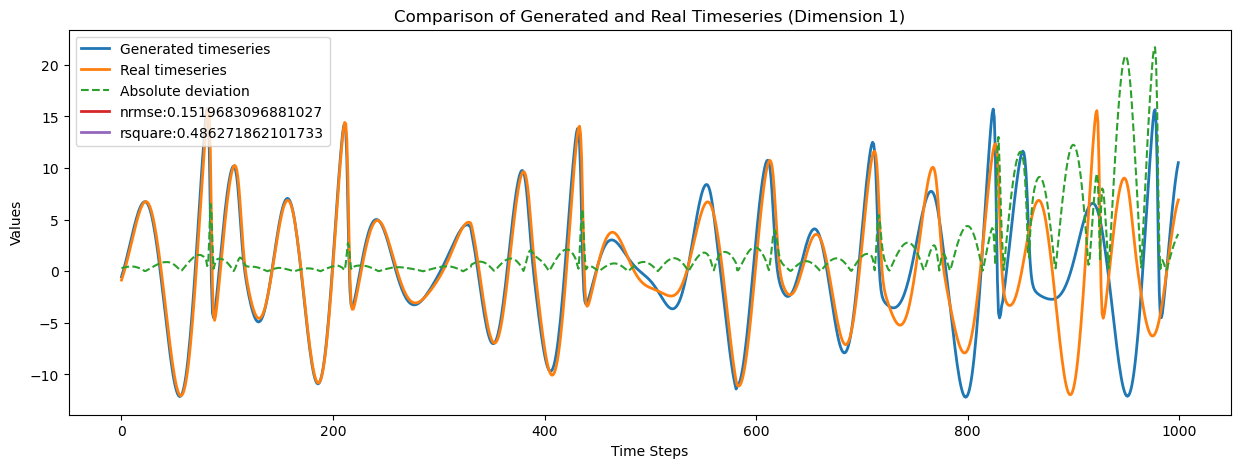
\includegraphics[width=0.8\textwidth]{Fig/custard1.png}
            \label{custard1.png} % ラベルを付ける(参照する場合に使用)
        \end{figure}
        \vspace{-1.0cm}

        \begin{figure}
            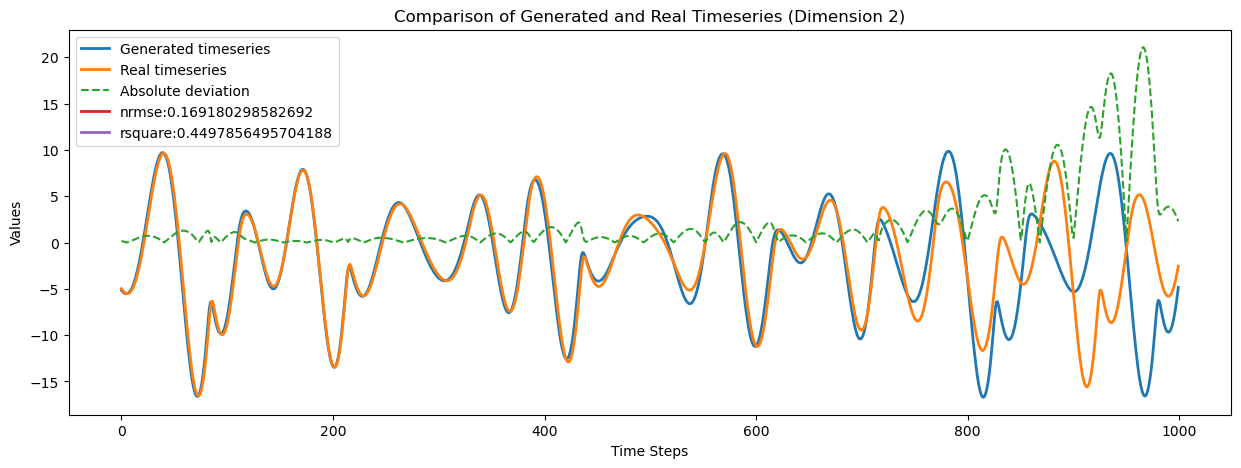
\includegraphics[width=0.8\textwidth]{Fig/custard2.png}
            \label{custard2.png} % ラベルを付ける(参照する場合に使用)
        \end{figure}
        \vspace{-1.0cm}

        \begin{figure}
            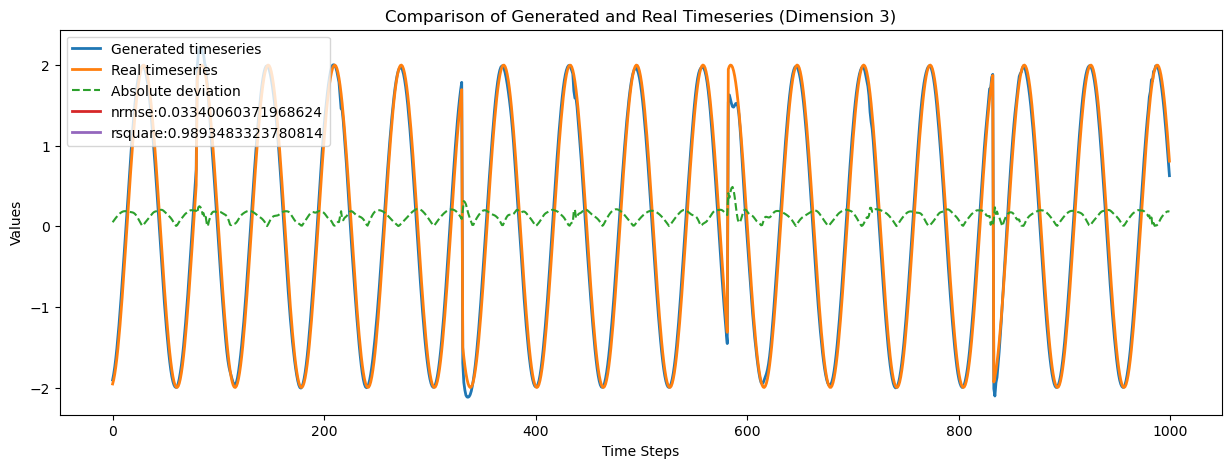
\includegraphics[width=0.8\textwidth]{Fig/custard3.png}
            \label{custard_3.png} % ラベルを付ける(参照する場合に使用)
            \caption{$x,\ y,$ 外力の予測\\ $z$ は学習・予測に用いられていない}
        \end{figure}
        \vspace{-1.0cm}
        \end{minipage}
    \begin{minipage}{0.5\textwidth}
        \begin{figure}
            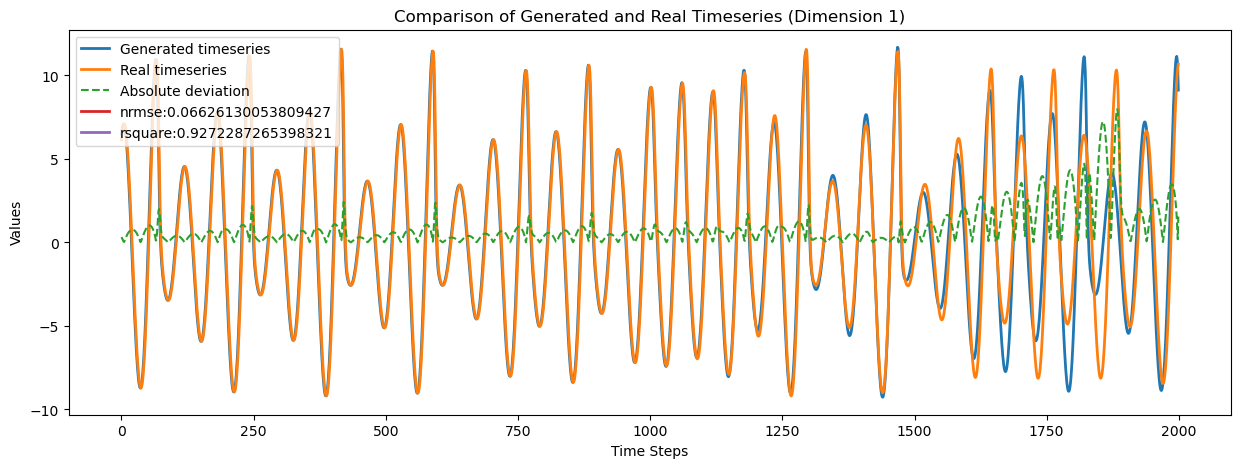
\includegraphics[width=0.8\textwidth]{Fig/rossler_+sin_1.png}
            \label{rossler_+sin_1.png} % ラベルを付ける(参照する場合に使用)
        \end{figure}
        \vspace{-1.0cm}
        \begin{figure}
            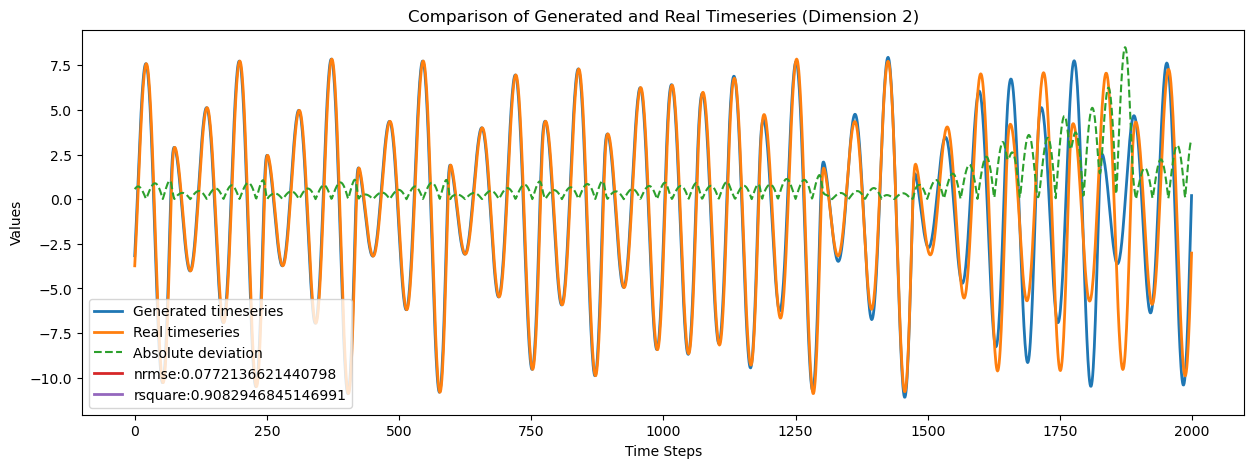
\includegraphics[width=0.8\textwidth]{Fig/rossler_+sin_2.png}
            \label{rossler_+sin_2.png} % ラベルを付ける(参照する場合に使用)
        \end{figure}
        \vspace{-1.0cm}
        \begin{figure}
            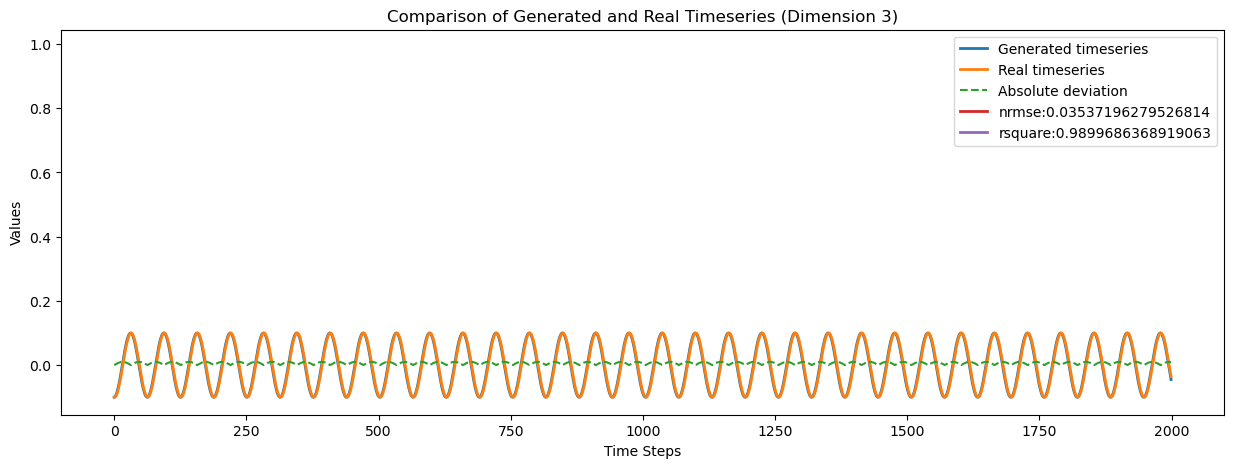
\includegraphics[width=0.8\textwidth]{Fig/rossler_+sin_3.png}
            \label{rossler_+sin_3.png} % ラベルを付ける(参照する場合に使用)
            \caption{参考:外力が $A \sin (t)$ のとき\\予測精度は高くなる}
        \end{figure}
    \end{minipage}
\end{frame}

\begin{frame}{位相シフトのある周期外力を持つRösslerモデル (2/2)}    
    \begin{minipage}{0.49\textwidth}
        \begin{figure}
            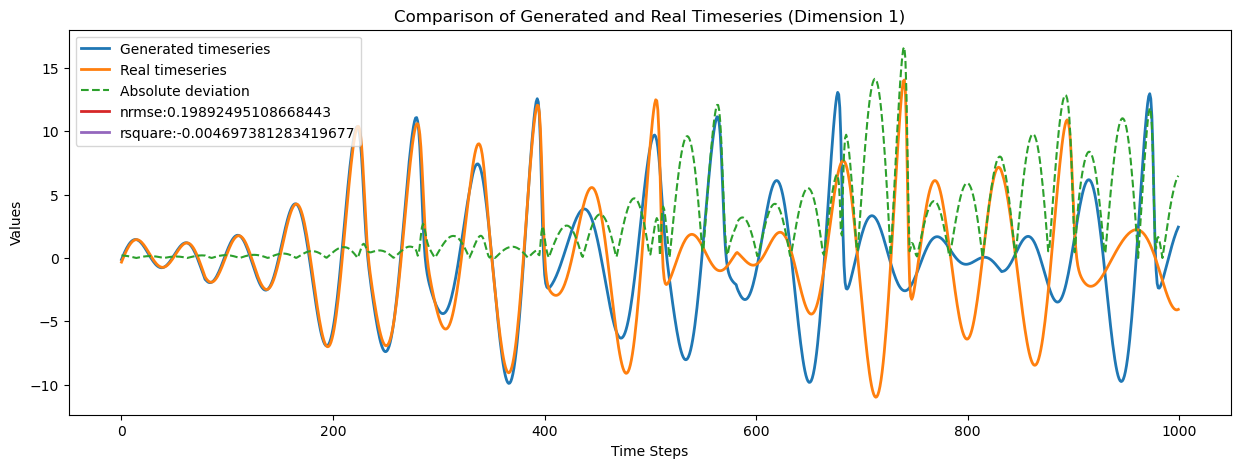
\includegraphics[width=0.8\textwidth]{Fig/custard_1.png}
            \label{custard_1.png} % ラベルを付ける(参照する場合に使用)
        \end{figure}
        \vspace{-1.0cm}

        \begin{figure}
            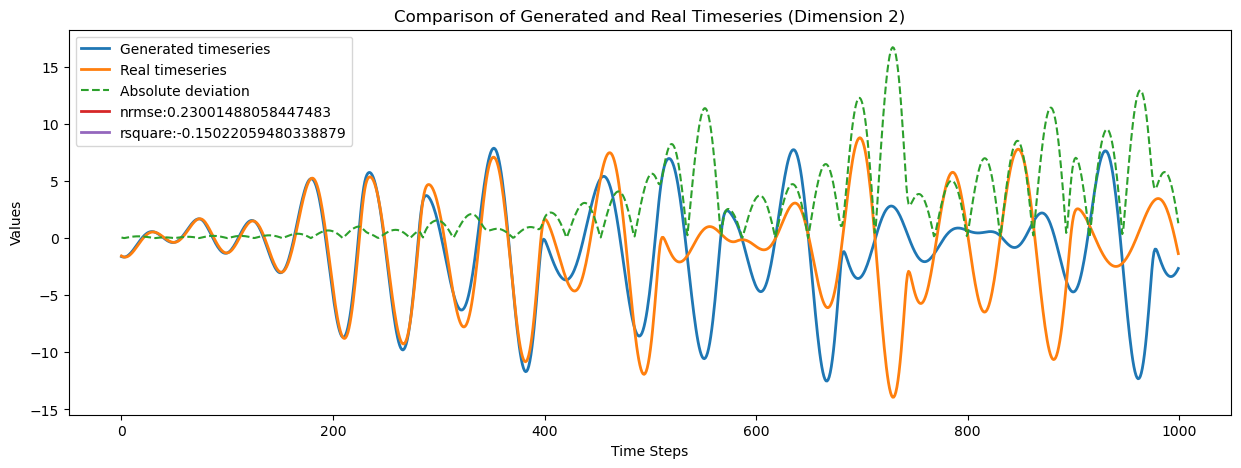
\includegraphics[width=0.8\textwidth]{Fig/custard_2.png}
            \label{custard_2.png} % ラベルを付ける(参照する場合に使用)
        \end{figure}
        \vspace{-1.0cm}

        \begin{figure}
            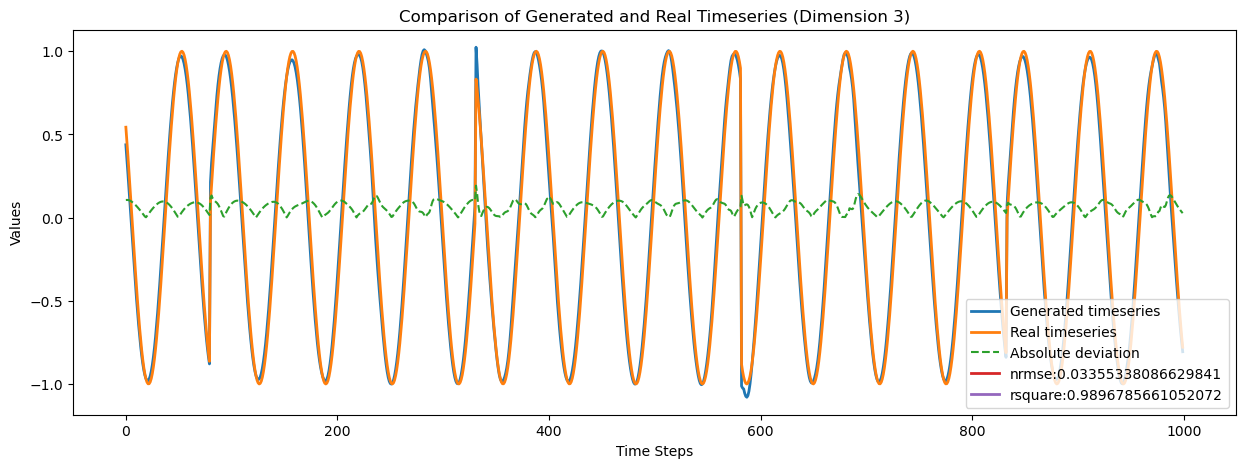
\includegraphics[width=0.8\textwidth]{Fig/custard_3.png}
            \label{custard_3.png} % ラベルを付ける(参照する場合に使用)
            \caption{異なる位相シフトに対しても同じReservoirで予測が可能}
        \end{figure}
        \vspace{-1.0cm}
        \end{minipage}

    \begin{minipage}{0.4\textwidth}
        
    \end{minipage}
\end{frame}
\begin{frame}{まとめと今後の展望}        
    \begin{minipage}{0.5\textwidth}
        まとめ:
        \begin{itemize}
            \item 位相シフトのある周期外力付きのRossler方程式の観測できる変数が限られている場合においても,Reserviorを用いた予測が可能である.
            \item 同じReservoirを使って未知の外力がある場合に対しても期間は短くなってしまうが予測は可能である.
        \end{itemize}
        \end{minipage}
    \begin{minipage}{0.49\textwidth}
        今後の展望:
        \begin{itemize}
            \item より複雑な未知の外力がある場合でも予測できるReservoir \begin{itemize}
                \item より複雑な構造を持つReservoirを設計する.
            \end{itemize}
            \item 観測できない変数があり外力があるような力学系の予測に対して,理論的な基盤を与える.
            \begin{itemize}
                \item 幾何学的な方向:Taken's embedding theorem
                \item 解析的な方向:Lyapunov function
            \end{itemize}
        \end{itemize}
    \end{minipage}
\end{frame}
